
\subsection{Estimation des coûts}

Nous indiquons ici le temps dédié à chacune des étapes du projet des deux sous-groupes suivi du temps consacré à la mise en commun de ces deux sous-parties.

\subsubsection{Automates}

\begin{flushleft}
\begin{tabular}{|l|c|r|}
  \hline
   Étape & Volume horaire \\
  \hline
  Travail initial sur les fichiers .an & 4h \\
     \hline
  Expressions régulières & 4h \\
  \hline
  Représentations visuelles des automates avec p5.js & ??h\\
  \hline
    Passage aux courbes de Bézier & ??h \\
  \hline
    Déplacement des arcs avec onmouse & ??h\\
  \hline
   Prise en main et calcul des overBox  & 6h \\
  \hline
   Affichage des transitions avec mousePressed() & 8h \\
    \hline
 \end{tabular}
 \end{flushleft}

Au total, nous avons consacré environ \textbf{??} heures pour cette sous-partie. 

\subsubsection{Graphes}

\begin{flushleft}
\begin{tabular}{|l|c|r|}
  \hline
   Étape & Volume horaire \\
  \hline
  Travail initial sur les fichiers .an & 4h \\
     \hline
  Expressions régulières & 4h \\
  \hline
  Représentations visuelles des automates avec p5.js & ??h\\
  \hline
    Passage aux courbes de Bézier & ??h \\
  \hline
    Déplacement des arcs avec onmouse & ??h\\
  \hline
   Prise en main et calcul des overBox  & 6h \\
  \hline
   Affichage des transitions avec mousePressed() & 8h \\
    \hline
 \end{tabular}
 \end{flushleft}

Au total, nous avons consacré environ \textbf{??} heures pour cette sous-partie. 
  
\subsubsection{Mise en commun}

\begin{flushleft}
\begin{tabular}{|l|c|r|}
  \hline
   Étape & Volume horaire \\
  \hline
 Lecture synchrone des fichiers & ??h \\
    \hline
 Rédaction du rapport & ??h \\
 \hline
    
 \end{tabular}
 \end{flushleft}

Au total, nous avons consacré environ \textbf{??} heures pour cette sous-partie.
\bigbreak
Ainsi, ce projet de groupe a été réalisé en \textbf{??} heures de travail. 
  
  
\bigbreak
\bigbreak
\subsection{Difficultés rencontrées}
\bigbreak

\subsubsection{Récupération des données depuis les fichiers .an}
Concernant la partie automates, notre première difficulté fut de récupérer les données des automates à partir des fichiers .an fournis:
\newpage
\begin{figure}
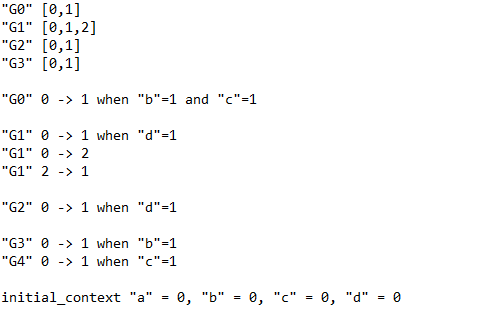
\includegraphics[scale=1]{images/fichier_an.PNG} 
\caption{Exemple de fichier .an}
\end{figure}
Nous avons au départ opté pour la méthode naïve de lire chacune des lignes et d'utiliser la méthode split (selon "when", "and" et "-") mais cette méthode cesse de fonctionner si  il y a plus de 10 automates puisque avoir "G10" au lieu de "G9" décalerait d'une case notre récupération naïve et de même si une transition à deux chiffres prenait place ("b" = 10 au lieu de "b" = 9). 
\newline
Nous avons donc préféré abandonné cette méthode malgré le temps consacré pour utiliser des expressions régulières, méthode bien plus robuste que la précédente.


\subsubsection{Déplacement des courbes}
Toujours dans la partie automates, une autre difficulté rencontrée fut de réussir à pouvoir déplacer les arcs, fonctionnalité nécessaire dès qu'il y a plus de $3$ arcs (représentant les transitions) arrivant ou sortant d'un état puisque la lecture devient alors très pénible:
\newpage
\begin{figure}
  \centering
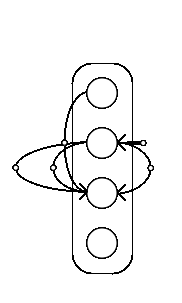
\includegraphics[scale=1]{images/arcs.PNG} 
\caption{Etats surchargés}
\end{figure}
La solution retenue pour rendre ces automates plus lisibles fut de rendre possible le déplacement de ces arcs: l'utilisateur peut ainsi remanier la figure à son goût. Cependant, il fut nécessaire de ré-écrire une portion conséquente du code d'affichage des automates car les méthodes d'affichage initiales écrites en utilisant la fonction \textbf{arc} de p5.js sont incompatibles avec le déplacement conçu par les méthodes \textbf{onmouse}. Ainsi, notre code final utilise les courbes de Bézier pour l'affichage des transitions.


\bigbreak
\subsubsection{Affichage des transitions}
Le dernier obstacle majeur de la partie automates a été celui de l'affichage des transitions puisque l'on voulait initialement que l'affichage des transitions ne s'affichent que lorsque l'utilisateur survole avec sa souris l'état concerné et que ces affichages suivent les arcs déplaçables: 
\begin{figure}
  \centering
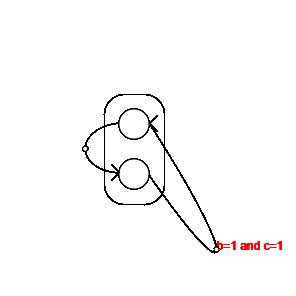
\includegraphics[scale=1]{images/transitions.png} 
\caption{La transition suit l'arc}
\end{figure}
Nous avons du consacré beaucoup de temps pour trouver une solution parmi la documentation souvent très absconse de p5.js et il a fallu ré-écrire cette fonctionnalité à chaque fois que la représentation visuelle des automates et de leurs arcs a été changée. Nous avons finalement retenu le principe de l'overBox: on construit un périmètre autour de l'arc et dès que l'utilisateur passe la souris dans ce périmètre, la transition s'affiche.
